\documentclass{optima}\usepackage[]{graphicx}\usepackage[]{color}
%% maxwidth is the original width if it is less than linewidth
%% otherwise use linewidth (to make sure the graphics do not exceed the margin)
\makeatletter
\def\maxwidth{ %
  \ifdim\Gin@nat@width>\linewidth
    \linewidth
  \else
    \Gin@nat@width
  \fi
}
\makeatother

\definecolor{fgcolor}{rgb}{0.345, 0.345, 0.345}
\newcommand{\hlnum}[1]{\textcolor[rgb]{0.686,0.059,0.569}{#1}}%
\newcommand{\hlstr}[1]{\textcolor[rgb]{0.192,0.494,0.8}{#1}}%
\newcommand{\hlcom}[1]{\textcolor[rgb]{0.678,0.584,0.686}{\textit{#1}}}%
\newcommand{\hlopt}[1]{\textcolor[rgb]{0,0,0}{#1}}%
\newcommand{\hlstd}[1]{\textcolor[rgb]{0.345,0.345,0.345}{#1}}%
\newcommand{\hlkwa}[1]{\textcolor[rgb]{0.161,0.373,0.58}{\textbf{#1}}}%
\newcommand{\hlkwb}[1]{\textcolor[rgb]{0.69,0.353,0.396}{#1}}%
\newcommand{\hlkwc}[1]{\textcolor[rgb]{0.333,0.667,0.333}{#1}}%
\newcommand{\hlkwd}[1]{\textcolor[rgb]{0.737,0.353,0.396}{\textbf{#1}}}%
\let\hlipl\hlkwb

\usepackage{framed}
\makeatletter
\newenvironment{kframe}{%
 \def\at@end@of@kframe{}%
 \ifinner\ifhmode%
  \def\at@end@of@kframe{\end{minipage}}%
  \begin{minipage}{\columnwidth}%
 \fi\fi%
 \def\FrameCommand##1{\hskip\@totalleftmargin \hskip-\fboxsep
 \colorbox{shadecolor}{##1}\hskip-\fboxsep
     % There is no \\@totalrightmargin, so:
     \hskip-\linewidth \hskip-\@totalleftmargin \hskip\columnwidth}%
 \MakeFramed {\advance\hsize-\width
   \@totalleftmargin\z@ \linewidth\hsize
   \@setminipage}}%
 {\par\unskip\endMakeFramed%
 \at@end@of@kframe}
\makeatother

\definecolor{shadecolor}{rgb}{.97, .97, .97}
\definecolor{messagecolor}{rgb}{0, 0, 0}
\definecolor{warningcolor}{rgb}{1, 0, 1}
\definecolor{errorcolor}{rgb}{1, 0, 0}
\newenvironment{knitrout}{}{} % an empty environment to be redefined in TeX

\usepackage{alltt}
\usepackage[sc]{mathpazo}
\usepackage[T1]{fontenc}
\usepackage{geometry}
\usepackage[backend=bibtex]{biblatex}
\IfFileExists{upquote.sty}{\usepackage{upquote}}{}
\begin{document}

\head{Dirk Schumacher}{Mixed integer linear programming in R with \emph{ompr}}



\noindent
R \cite{r} is a popular language and computational environment among statisticians. In recent years R has gained a lot of popularity in other disciplines as well. With over 11,000 packages on CRAN \cite{cran}, the R package repository, there is a package for almost every problem. And of course, packages for solving mixed integer linear programs are also available. R as a language makes it easy to create domain specific languages through metaprogramming using so-called non-standard evaluation \cite{advancedr}.

\emph{ompr} (the optimization modelling package) \cite{ompr} is an attempt to develop an algebraic modelling language within R. The goal is to create a modelling API that uses idiomatic R and integrates well with other popular packages, such as \emph{dplyr} for data processing. \emph{ompr} models are solver-independent and currently support mixed integer linear programming problems. It works on all platforms supported by R (Linux, MacOS and Windows). Compared to other modelling languages it comes closest to \emph{JuMP} \cite{jump} for \emph{julia} but is currently more limited in terms of features and scope. In fact \emph{JuMP} inspired me to build \emph{ompr}.

The features of \emph{ompr} are best described by modelling a mixed integer linear program in R. As an example for this article we model a \emph{warehouse location problem} where we would like to find the cost optimal location and number of warehouses and the assignment of customers to those hubs.

\begin{figure}[h]
\begin{equation*}
\begin{array}{lll@{}}
\text{min}  & \displaystyle\sum\limits_{i=1}^{n}\sum\limits_{j=1}^{m}\operatorname{tc}_{i,j} \cdot x_{i, j} & +  \sum\limits_{j=1}^{m}\operatorname{fc}_{j} \cdot y_{j}\\
\text{subject to} & \displaystyle\sum\limits_{j=1}^{m}   x_{i, j} = 1  & \forall\,i=1 ,\ldots, n\\
                  & \displaystyle x_{i, j} \leq y_j,  & \forall\,i=1 ,\ldots, n,\,j=1 ,\ldots, m\\
                 &                                                x_{i,j} \in \{0,1\} &\forall\,i=1 ,\ldots, n,\,j=1 ,\ldots, m\\
                 &                                                y_{j} \in \{0,1\} &\forall\,j=1 ,\ldots, m
\end{array}
\end{equation*}
\caption{A warehouse location problem as an illustrative example. $n$ customers need to be assigned to exactly one of at most $m$ warehouses. Setting up a warehouse $y_j=1$ has a fixed cost of $\operatorname{fc}_j>0$ and assigning a customer to a warehouse $x_{i,j}=1$ leads to travel cost of $\operatorname{tc}_{i,j}>0$.}
\end{figure}



Every \emph{ompr} model starts with an empty model to which necessary elements (like variables, constraints and an objective function) are added. Expressions can be mixed with  variables defined in the general environment. For example in the model below the functions $\operatorname{tc}$ and $\operatorname{fc}$ are not part of the optimization problem, but are regular R functions defined in the environment. Like other algebraic domain specific languages, equations can be written down directly and the package takes care of transforming these to the required format for the API of the solver.

\begin{figure}[h]
\begin{small}
\begin{knitrout}
\definecolor{shadecolor}{rgb}{0.969, 0.969, 0.969}\color{fgcolor}\begin{kframe}
\begin{alltt}
\hlkwd{library}\hlstd{(ompr)}
\hlstd{model} \hlkwb{<-} \hlkwd{MIPModel}\hlstd{()} \hlopt
  \hlkwd{add_variable}\hlstd{(x[i, j],} \hlkwc{i}\hlstd{=}\hlnum{1}\hlopt{:}\hlstd{n,} \hlkwc{j}\hlstd{=}\hlnum{1}\hlopt{:}\hlstd{m,} \hlkwc{type}\hlstd{=}\hlstr{"binary"}\hlstd{)} \hlopt
  \hlkwd{add_variable}\hlstd{(y[j],} \hlkwc{j}\hlstd{=}\hlnum{1}\hlopt{:}\hlstd{m,} \hlkwc{type}\hlstd{=}\hlstr{"binary"}\hlstd{)} \hlopt
  \hlkwd{set_objective}\hlstd{(}
    \hlkwd{sum_expr}\hlstd{(}\hlkwd{tc}\hlstd{(i, j)} \hlopt{*} \hlstd{x[i, j],} \hlkwc{i}\hlstd{=}\hlnum{1}\hlopt{:}\hlstd{n,} \hlkwc{j}\hlstd{=}\hlnum{1}\hlopt{:}\hlstd{m)} \hlopt{+}
    \hlkwd{sum_expr}\hlstd{(}\hlkwd{fc}\hlstd{(j)} \hlopt{*} \hlstd{y[j],} \hlkwc{j}\hlstd{=}\hlnum{1}\hlopt{:}\hlstd{m),}
    \hlkwc{sense} \hlstd{=} \hlstr{"min"}\hlstd{)} \hlopt
  \hlkwd{add_constraint}\hlstd{(}\hlkwd{sum_expr}\hlstd{(x[i, j],} \hlkwc{j}\hlstd{=}\hlnum{1}\hlopt{:}\hlstd{m)} \hlopt{==} \hlnum{1}\hlstd{,} \hlkwc{i}\hlstd{=}\hlnum{1}\hlopt{:}\hlstd{n)} \hlopt
  \hlkwd{add_constraint}\hlstd{(x[i, j]} \hlopt{<=} \hlstd{y[j],} \hlkwc{i}\hlstd{=}\hlnum{1}\hlopt{:}\hlstd{n,} \hlkwc{j}\hlstd{=}\hlnum{1}\hlopt{:}\hlstd{m)}
\end{alltt}
\end{kframe}
\end{knitrout}
\end{small}
\caption{The \emph{warehouse location problem} modeled with \emph{ompr} using so called pipes to chain together successive functions. }
\end{figure}

After an \emph{ompr} model is built, it can be passed to a solver. Within \emph{ompr} a solver is simply a function mapping a model to a solution. In this case the GNU Linear Programming Kit \cite{glpk} is used to find an optimal solution. To support most popular solvers out of the box, the package \emph{ompr.roi} can be used. It makes it possible to use any solver supported by the \emph{R optimization infrastructure} (\emph{ROI}) packages \cite{roi}. \emph{ROI} gives access to many open source (\emph{CLP}, \emph{GLPK}, \emph{lpsolve}, \emph{Symphony}) and commercial solvers (\emph{CPLEX}, \emph{Gurobi}) through a standardized interface.

\begin{figure}[h]
\begin{small}
\begin{knitrout}
\definecolor{shadecolor}{rgb}{0.969, 0.969, 0.969}\color{fgcolor}\begin{kframe}
\begin{alltt}
\hlkwd{library}\hlstd{(ompr.roi)}
\hlkwd{library}\hlstd{(ROI.plugin.glpk)}
\hlstd{result} \hlkwb{<-} \hlkwd{solve_model}\hlstd{(model,} \hlkwd{with_ROI}\hlstd{(}\hlkwc{solver} \hlstd{=} \hlstr{"glpk"}\hlstd{))}
\hlstd{assignment} \hlkwb{<-} \hlkwd{get_solution}\hlstd{(result, x[i, j])}
\hlstd{warehouses} \hlkwb{<-} \hlkwd{get_solution}\hlstd{(result, y[i])}
\end{alltt}
\end{kframe}
\end{knitrout}
\end{small}
\caption{The model defined earlier is solved with the GNU Linear Programming Kit using the solver package \emph{ompr.roi} which offers access to a variety of open source and commercial solvers.}
\end{figure}

The result can then be further processed within the R ecosystem. For example using R's plotting facilities, we can plot the assignment (Figure \ref{fig:ompr_fig_warehouse}).


\begin{figure}[h]
\begin{knitrout}
\definecolor{shadecolor}{rgb}{0.969, 0.969, 0.969}\color{fgcolor}

{\centering 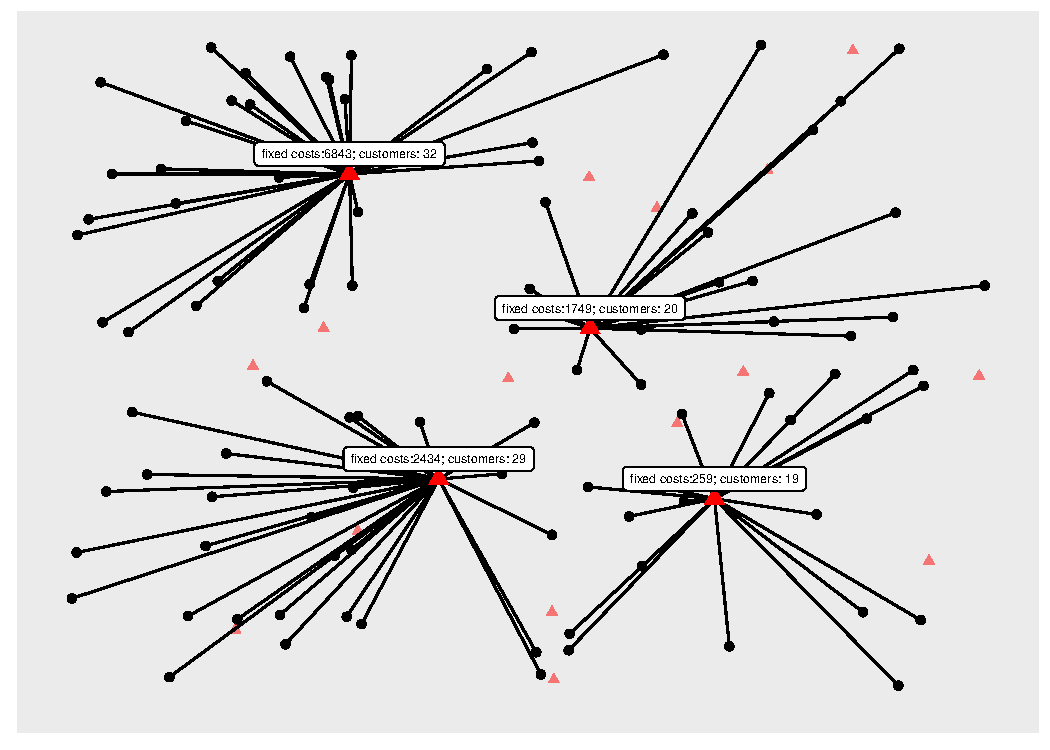
\includegraphics[width=\maxwidth]{figure/optima-figure-1} 

}



\end{knitrout}
\caption{A solution to the warehouse location problem generated by \emph{ggplot2} and \emph{ompr}.}
\label{fig:ompr_fig_warehouse}
\end{figure}

Currently \emph{ompr}'s cost of abstraction can be rather high for larger models, but this is something I plan to work on in the future. Up to now the focus has been on creating an idiomatic API for modelling mixed integer linear programs directly in R. \emph{ompr} as well as \emph{ompr.roi} are published on CRAN and developed on GitHub. The packages are open source and I encourage anyone to send feedback, ideas or code contributions. On the project's website \cite{ompr} I have compiled some articles showcasing the modelling features of the package and tutorials on how to model selected optimization problems in R with \emph{ompr}.

In my opinion a big advantage of modelling optimization problems in R is the ability to easily utilize other packages within the R ecosystem for data wrangling, statistics, (interactive) visualizations and reproducible research. For example, this article was generated in a completely reproducible manner with \emph{knitr} \cite{knitr} and the code shown here is the actual code that led to the output in Figure \ref{fig:ompr_fig_warehouse}; it is published on GitHub (\url{https://github.com/dirkschumacher/ompr-optima}) as well.


\begin{jinfo}
Dirk Schumacher, Berlin, Germany. \href{mailto:mail@dirk-schumacher.net}{\url{mail@dirk-schumacher.net}}

\end{jinfo}

\begin{thebibliography}{3}

\bibitem{advancedr}
Hadley Wickham.
\newblock Advanced R.
\newblock CRC Press, 2014.

\bibitem{r}
 R Development Core Team.
 \newblock R: A language and environment for statistical computing.
 \newblock R Foundation for Statistical Computing, Vienna, Austria. ISBN 3-900051-07-0, URL \url{https://www.R-project.org}, 2008.

\bibitem{ompr}
Dirk Schumacher.
\newblock ompr: optimization modelling package.
\newblock R package version 0.6, \url{https://cran.r-project.org/package=ompr}, 2017.

\bibitem{cran}
CRAN: The Comprehensive R Archive Network.
\newblock \url{https://cran.r-project.org/}, 2017-07-16.

\bibitem{roi}
Kurt Hornik and David Meyer and Florian Schwendinger and Stefan Theussl.
\newblock ROI: R Optimization Infrastructure.
\newblock R package version 0.2-1, \url{https://cran.r-project.org/package=ROI}, 2016.

\bibitem{jump}
Dunning, Iain and Joey Huchette and Miles Lubin.
\newblock JuMP: A modeling language for mathematical optimization.
\newblock SIAM Review 59.2 (2017): 295-320.

\bibitem{glpk}
GNU Linear Programming Kit.
\newblock \url{http://www.gnu.org/software/glpk/glpk.html}, 2017.

\bibitem{knitr}
Yihui Xie.
\newblock knitr: A General-Purpose Package for Dynamic Report Generation in R.
\newblock R package version 1.1, 2017.

\end{thebibliography}

\end{document}
